\chapter{Configuring a Hadoop Cluster}\label{chap:3}
In this chapter, we will cover:

\begin{itemize}
  \item Choosing a Hadoop version
  \item Configuring Hadoop in pseudo-distributed mode
  \item Configuring Hadoop in fully-distributed mode
  \item Validating Hadoop installation
  \item Installing ZooKeeper
  \item Installing HBase
  \item Installing Hive
  \item Installing Pig
  \item Installing Mahout
\end{itemize}

\section{Choosing a Hadoop version}
As an open source project, Hadoop has been under active development over the past a few years. New versions are being released regularly. These new releases either fix bugs contributed by the community, leading to a more stable Hadoop software stack or add new features for the purpose of more full-fledged, enterprise class distribution.

In this section, we are going to review the release\index{release} history of Hadoop, pointing out features of these releases. More importantly, we will give tips on choosing a proper Hadoop distribution.

\subsection*{Getting ready}
In General, the release version number of a Hadoop distribution consists of three parts: the version number\index{version number}, the major revision number\index{major revision number} and the minor revision number\index{minor revision number}. A Hadoop release version can be described with the following figure:
\begin{figure}[ht]
  \centering
  
\includegraphics[width=.5\textwidth]{figs/5163os_03_01.png}
  \caption{Structure of a Hadoop release version}\label{fig:hadoop.release}
\end{figure} 
Sometimes, the revision number can have a fourth part, for example 0.20.203.0, but this is relatively rare.
\subsection*{How to do it...}
The following table shows features of major Hadoop releases:
\begin{table}[h]
  \centering
  \begin{tabular}{l|l|l|l|l}
    \toprule
    \textbf{Feature or Version} & \textbf{2.x.y} & \textbf{1.1.x} & \textbf{0.23.x} & \textbf{0.20.x} \\ \midrule
    Stable &  & Yes &  & Yes \\
    MRv1 &  & Yes &  & Yes \\
    MRv2 & Yes &  & Yes & \\
    Kerberos Security & Yes & Yes & Yes & \\
    HDFS federation & Yes &  & Yes & \\
    NameNode HA & Yes &  & Yes &  \\
    HDFS append & Yes & Yes & Yes & \\
    HDFS symbolic Links & Yes & Yes & Yes & \\ \bottomrule
  \end{tabular}
\end{table}
The table tells us that Hadoop is evolving rapidly, with new features such as security, HDFS federation\index{HDFS federation} and NameNode HA\index{NameNode HA} being added over time. Another lesson we can learn from the table is that the most recent stable release version 1.1.x does not contain all the features. And although release version 2.0.x is the most feature rich Hadoop release, it is still in alpha state requiring further improvements.

So, which version should I choose for my deployment? Generally, we need to consider the following two properties: stability and features. For a production deployment, we definitely want to deploy a stable release and we also want to use the release that contains all the required features. Clearly, our current optimal and only choice is version 1.1.x, or specifically version 1.1.2 as of this book writing.

\subsection*{See also}
\begin{itemize}
  \item More information about Hadoop releases can be found at \href{http://hadoop.apache.org/releases.html}{Hadoop @ Apache}
\end{itemize}

\section{Configuring Hadoop in pseudo-distributed mode}
Pseudo-distributed mode\index{Pseudo-distributed mode} refers to a Hadoop cluster configuration that contains only one node. This mode can be helpful for debugging and validation purposes. In this recipe, we will outline steps to configure Hadoop in pseudo-distributed mode.
\subsection*{Getting ready}
Before configuring Hadoop in pseudo-distributed mode, we assume that we have a machine, for example the master node of the Hadoop cluster, with Linux installed. And all the necessary tools have been installed and properly configured.

The most important dependent software is Java, which is the programming language and library that Hadoop is based on. To check that Java has been properly installed,
we can use the following command:
\verb|$ java -version|

You should have output similar to the following:
\lstset{style=bashstyle}
\begin{lstlisting}[caption=Java Version Information]
java version "1.7.0_13"
Java(TM) SE Runtime Environment (build 1.7.0_13-b20)
Java HotSpot(TM) 64-Bit Server VM (build 23.7-b01, mixed mode)
If you have installed OpenJDK other than the Oracle's official Java, the output will be similar to the following:
Java version "1.7.0_09-icedtea"
OpenJDK Runtime Environment (fedora-2.3.4.fc17-x86_64)
OpenJDK 64-Bit Server VM (build 23.2-b09, mixed mode)
\end{lstlisting}
If you have installed OpenJDK, please refer to recipe \emph{Installing Java and other tools} of Chapter 2, Preparing for Hadoop installation.

Download the desired Hadoop distribution. In this book, we assume to use Hadoop release 1.1.2.

To download a Hadoop release from one \href{http://www.apache.org/dyn/closer.cgi/hadoop/common/}{mirror site}, choose the proper mirror site (or use the suggested link on top of the mirror). Start download by clicking the proper Hadoop release. We suggest downloading a gzip archived file with file name ending with tar.gz.

Alternatively, we can download a Hadoop release with the following command under Linux:
\lstset{style=bashstyle}
\begin{lstlisting}
wget http://mirror.quintex.com/apache/hadoop/common/hadoop-1.1.2/hadoop-1.1.2.tar.gz -P ~
\end{lstlisting}

Last, we assume that ssh password-less login has been properly configured.
\subsection*{How to do it...}
Use the following recipe to configure Hadoop in pseudo-distributed mode:

Copy the Hadoop archive to \verb|/usr/local| directory:\\
\verb|sudo cp hadoop-1.1.2.tar.gz /usr/local|

Decompress the Hadoop package archive: \\
\verb|cd /usr/local| \\
\verb|sudo tar xvf hadoop-1.1.2.tar.gz|

The uncompressed archive file will contain the following files and folders:
\lstset{style=bashstyle}
\begin{lstlisting}[caption=Content from the uncompressed Hadoop package.]
CHANGES.txt  c++                     hadoop-examples-1.1.2.jar     lib
LICENSE.txt  conf                    hadoop-minicluster-1.1.2.jar  libexec
NOTICE.txt   contrib                 hadoop-test-1.1.2.jar         sbin
README.txt   hadoop-ant-1.1.2.jar    hadoop-tools-1.1.2.jar        share
bin          hadoop-client-1.1.2.jar ivy                           src
build.xml    hadoop-core-1.1.2.jar   ivy.xml                       webapps
\end{lstlisting}
The folder contains several jar files and folders such as bin, sbin and conf. Jar files hadoop-core-1.1.2.jar and hadoop-tools-1.1.2.jar contain the core classes of Hadoop. File hadoop-examples-1.1.2.jar and hadoop-test-1.1.2.jar contains sample MapReduce jobs.

Folder conf contains cluster configuration files, folder bin contains commands and scripts to start and stop a cluster and folder sbin contains scripts to do specific tasks.

Make a soft link for Hadoop root directory. \\
\verb|$ sudo ln -s hadoop-1.1.2 hadoop|

Use your favorite text editor to open file ~/.bashrc and add the following contents: 
\begin{verbatim}
export JAVA_HOME=/usr/java/latest
export HADOOP_HOME=/usr/local/hadoop
export PATH=$PATH:$JAVA_HOME/bin:HADOOP_HOME/bin
\end{verbatim}

We are assuming Oracle Java has been installed under directory /usr/java/latest. \\
Source file ~/.bashrc with command: \\
\verb|$ . ~/.bashrc|

Use your favorite text editor to open file \verb|$HADOOP_HOME/conf/hadoop-env.sh| and change the \verb|JAVA_HOME| environment variable to: \\
\verb|export JAVA_HOME=/usr/Java/latest|

Use your favorite text editor to open file \verb|$HADOOP_HOME/conf/core-site.xml| and add the following content:
\lstset{style=bashstyle}
\begin{lstlisting}[caption=Content of the core-site.xml file]
<configuration>
  <property>
    <name>fs.default.name</name>
    <value>hdfs://localhost:54310</value>
  </property>

  <property>
    <name>mapred.job.tracker</name>
    <value>localhost:54311</value>
  </property>

  <property>
    <name>hadoop.tmp.dir</name>
    <value>/hadoop/tmp/</value>
  </property>
</configuration>
\end{lstlisting}

Use your favorite text editor to open file \verb|$HADOOP_HOME/conf/hdfs-site.xml| and add the following content to the file:
\begin{lstlisting}[caption=Content of file hdfs-site.xml]
<configuration>
  <property>
    <name>dfs.replication</name>
    <value>2</value>
  </property>

  <property>
    <name>dfs.data.dir</name>
    <value>/hadoop/data/</value>
  </property>
</configuration>
\end{lstlisting}

Use your favorite text editor to open file \verb|$HADOOP_HOME/conf/mapred-site.xml| and add the following content:
\begin{lstlisting}[caption=Content of file mapred-site.xml]
<configuration>
  <property>
    <name>mapred.system.dir</name>
    <value>/hadoop/mapred</value>
  </property>
</configuration>
\end{lstlisting}

Ask localhost to run SecondaryNameNode daemon with command: \\
\verb|$ sudo echo ``localhost'' > $HADOOP_HOME/conf/masters|

Configure localhost as the single slave node with command: \\
\verb|$ sudo echo "localhost" > $HADOOP_HOME/conf/slaves|

Use the following steps to start and stop a Hadoop cluster:

Format the HDFS filesystem from NameNode with the following command: \\
\verb|$ hadoop namenode -format|

We will get output similar to the following:
\lstset{style=bashstyle}
%%\begin{Verbatim}[fontfamily=courier,fontsize=\scriptsize]
\begin{lstlisting}[caption=NameNode formatting output]
13/02/14 01:43:12 INFO namenode.NameNode: STARTUP_MSG:
/************************************************************
STARTUP_MSG: Starting NameNode
STARTUP_MSG:   host = localhost/127.0.0.1
STARTUP_MSG:   args = [-format]
STARTUP_MSG:   version = 1.1.2
STARTUP_MSG:   build = https://svn.apache.org/repos/asf/hadoop/common/branches/branch-1.0 -r 1393290; compiled by 'hortonfo' on Wed Oct  3 05:13:58 UTC 2012
************************************************************/
13/02/14 01:43:13 INFO util.GSet: VM type       = 64-bit
13/02/14 01:43:13 INFO util.GSet: 2% max memory = 17.77875 MB
13/02/14 01:43:13 INFO util.GSet: capacity      = 2^21 = 2097152 entries
13/02/14 01:43:13 INFO util.GSet: recommended=2097152, actual=2097152
13/02/14 01:43:13 INFO namenode.FSNamesystem: fsOwner=shumin
13/02/14 01:43:13 INFO namenode.FSNamesystem: supergroup=supergroup
13/02/14 01:43:13 INFO namenode.FSNamesystem: isPermissionEnabled=true
13/02/14 01:43:13 INFO namenode.FSNamesystem: dfs.block.invalidate.limit=100
13/02/14 01:43:13 INFO namenode.FSNamesystem: isAccessTokenEnabled=false accessKeyUpdateInterval=0 min(s), accessTokenLifetime=0 min(s)
13/02/14 01:43:13 INFO namenode.NameNode: Caching file names occuring more than 10 times
13/02/14 01:43:13 INFO common.Storage: Image file of size 112 saved in 0 seconds.
13/02/14 01:43:14 INFO common.Storage: Storage directory /hadoop/tmp/dfs/name has been successfully formatted.
13/02/14 01:43:14 INFO namenode.NameNode: SHUTDOWN_MSG:
/************************************************************
SHUTDOWN_MSG: Shutting down NameNode at localhost/127.0.0.1
************************************************************/
\end{lstlisting}

Start the HDFS daemons with command: \\
\verb|$ start-dfs.sh|

We will get output similar to the following:
\lstset{style=bashstyle}
\begin{lstlisting}[caption=Output for starting the HDFS cluster.]
starting namenode, logging to /usr/local/hadoop/libexec/../logs/hadoop-hduser-namenode-localhost.out
localhost: starting datanode, logging to /usr/local/hadoop/Hadoop/libexec/../logs/hadoop-hduser-datanode-localhost.out
localhost: starting secondarynamenode, logging to /usr/local/hadoop/libexec/../logs/hadoop-hduser-secondarynamenode-localhost.out
\end{lstlisting}
The output shows that the following HDFS daemons have been started: \emph{NameNode}, \emph{DataNode} and \emph{SecondaryNameNode}.

Start the MapReduce daemons with command: \\
\verb|$ start-mapred.sh|

The output will be similar to:
\lstset{style=bashstyle}
\begin{lstlisting}[caption=Output message when starting the MapReduce cluster]
starting jobtracker, logging to /usr/local/hadoop/libexec/../logs/hadoop-hduser-jobtracker-localhost.out
localhost: starting tasktracker, logging to /usr/local/hadoop/libexec/../logs/hadoop-hduser-tasktracker-localhost.out
\end{lstlisting}

The output shows that the following MapReduce daemons have been started: JobTracker and TaskTracker.

With the jps command, we can get a list of all running daemons:
\lstset{style=bashstyle}
\begin{lstlisting}
10984 SecondaryNameNode
11272 TaskTracker
11144 JobTracker
26966 NameNode
10855 DataNode
27183 Jps
\end{lstlisting}

So far, all the Hadoop daemons have been started.

Stop the MapReduce daemons with command: \\
\verb|$ stop-mapred.sh|

Stop the HDFS daemons with command: \\
\verb|$ stop-hdfs.sh|

\subsection*{How it works...}
Under Unix-like operating systems, system runtime configurations and environment variables are specified via plain text files. These files are called run configuration file, meaning that they provide configurations when the program runs. For example, file .bashrc under a user's home directory is the run configuration file for bash shell. It will be sourced (loaded) automatically every time when a bash terminal is opened. So, in this file, we can specify commands and environment variables for a running bash environment.

\verb|.bashrc| OR \verb|.bash_profile|

Under Linux, the bash shell has two run configuration files for a user, \verb|.bashrc| and \verb|.bash_profile|. The difference between the two files is that \verb|.bash_profile| is executed for login shells, while \verb|.bashrc| for interactive non-login shells. More specifically, when we login to the system by entering username and password either locally or from a remote machine \verb|.bash_profile| will be executed and a bash shell process initialized. On the other hand, if we open a new bash terminal after logged into a machine or type the bash command from command line, file \verb|.bashrc| will be used for initialization before we see the command prompt on the terminal window. In this recipe, we used file \verb|.bashrc|, so that new configurations will be available after opening a new bash process. Alternatively, we can manually source a configuration file after it is created or changed with the source command.

The following table shows configuration files for configuring a Hadoop cluster in pseudo-distributed mode:
\begin{table}[h]
  \centering
\begin{tabular}{ll}  
    \toprule
    \textbf{File} & \textbf{Description} \\ \midrule
    hadoop-env.sh & Configures environment variable used by Hadoop. \\
    core-site.xml & Configures parameters for the whole Hadoop cluster. \\
    hdfs-site.xml & Configures parameters for HDFS and its clients. \\
    mapred-site.xml & Configures parameters for MapReduce and its clients. \\
    masters & Configures host machines for SecondaryNameNode. \\
    slaves & Configures a list of slave node hosts. \\ \bottomrule
  \end{tabular}
\end{table}

\begin{itemize}
  \item \emph{hadoop-env.sh} specifies environment variables for running Hadoop. For example, the home directory of Java installation \verb|JAVA_HOME| and those related to Hadoop runtime options and cluster logging etc.
  \item \emph{core-site.xml} specifies the URI of HDFS NameNode and MapReduce JobTracker. Value \url{hdfs://localhost:54310} of the fs.default.name property specifies the location of the default file system as HDFS on localhost using port 54310. We can specify other file system schemes such as local file system with \url{file:///home/hduser/hadoop} and amazon web service S3 with \url{s3://a-bucket/hadoop} etc. Value localhost:54311 of the mapred.job.tracker property specifies the URI of the cluster's JobTracker.
  \item \emph{hdfs-site.xml} specifies the HDFS related configurations. For example, dfs.replication configures the replication factor of data blocks on HDFS. For example, the value 2 specifies that each data block will be replicated twice on the file system. Property dfs.data.dir specifies the location of the data directory on the host Linux file system.
  \item \emph{mapred-site.xml} specifies configurations for the MapReduce framework. For example, we can configure the total number of jvm tasks, the number of map slots and reduce slots on a slave node and the amount of memory for each task etc.
  \item \emph{masters} file specifies hosts that will run a SecondaryNameNode daemon. In our single node configuration, we put localhost in this file. And a SecondaryNameNode daemon will be started on localhost, which has been verified with the jps command.
  \item slaves file specifies slave nodes that run tasks controlled by task trackers. In our pseudo-distributed mode configuration, localhost is the only slave node in the cluster.
\end{itemize}

Hadoop provides a number of bash scripts for convenience of starting and stopping a cluster. The following table shows these scripts:
\begin{description}
    \item{start-dfs.sh} Script to start HDFS daemons including NameNode, SecondaryNameNode and DataNode. A PID file will be created for each daemon process under default folder \${hadoop.tmp.dir}. For example, if user hduser is used to run the script, file /hadoop/tmp/hadoop-hduser-namenode.pid will be created for the NameNode daemon process.
    \item{stop-dfs.sh} Script to stop HDFS daemons. This command will try to find the PIDs of the HDFS daemons and kill the processes with the PIDs. So, if the PID file is missing, this script will not work.
    \item{start-mapred.sh} Script to start MapReduce daemons, including the JobTracker and TaskTrackers. Similar to start-hdfs.sh script, PIDs files will be created for each daemon process.
    \item{stop-mapred.sh} Script to stop Hadoop MapReduce daemons. Similar to stop-dfs.sh script, the script will try to find the PID files and then kill those processes.
    \item{start-all.sh} Equals to start-dfs.sh plus start-mapred.sh.
    \item{stop-all.sh} Equals to stop-dfs.sh plus stop-mapred.sh.
\end{description}
\subsection*{There's more...}
Currently, Hadoop is also available in rpm format. So we can use the following command to install Hadoop:
\lstset{style=bashstyle}
\begin{lstlisting}
$ sudo rpm -ivh http://www.poolsaboveground.com/apache/hadoop/common/stable/hadoop-1.1.2-1.x86_64.rpm
\end{lstlisting}

The locations of installed files will be different from the tar ball method. And we can check the file layout with command: \\
\verb|$ rpm -ql hadoop|

Then we can use the following command to configure a Hadoop cluster in single node: \\
\verb|$ sudo hadoop-setup-single-node.sh|
\subsection*{See also}
\begin{itemize}
  \item Configuring Hadoop in fully distributed mode
  \item Validating Hadoop installation in Chapter
\end{itemize}

\section{Configuring Hadoop in fully-distributed mode}
To configure a Hadoop cluster in fully-distributed mode\index{fully-distributed mode}, we need to configure all the master and slave machines. Although different from the pseudo-distributed mode, the configuration experience will be similar.  In this recipe, we will outline steps to configure Hadoop in fully-distributed mode.
\subsection*{Getting ready}
In this book, we propose to configure a Hadoop cluster with 1 master node and 5 slave nodes. The hostname of the master node is 1 and the hostnames of the slave nodes are: \textbf{slave1, slave2, slave3, slave4}, and \textbf{slave5}.

Before getting started, we assume that Linux has been installed on all the cluster nodes and we should validate password-less login with the following commands on the master node:
\lstset{style=bashstyle}
\begin{lstlisting}
$ ssh hduser@slave1
$ ssh hduser@slave2
...
\end{lstlisting}
Unlike the pseudo-distributed mode, configuring a Hadoop cluster in fully-distributed mode requires the successful configuration of all the nodes in the cluster. Otherwise, the cluster will not work as expected.

We should be cautious about the interconnection of the cluster nodes. Connection problems might be caused by configurations of firewalls, network and so on.
Assuming file \verb|$HADOOP_HOME/conf/slaves| contains hostnames of the slave nodes, we can use the following command to check the password-less login to all slave nodes from the master node: 
\lstset{style=bashstyle}
\begin{lstlisting}
for host in `cat $HADOOP_HOME/conf/slaves`; do
  echo "Testing ssh from master to node" $host
  ssh hduser@$host
done
\end{lstlisting}

\subsection*{How to do it...}
Use the following recipe to configure Hadoop in fully-distributed mode: \\
Login to the master node from administrator machine with command: \\
\verb|$ ssh hduser@master|

Copy the Hadoop archive to the \verb|/usr/local| directory:
\lstset{style=bashstyle}
\begin{lstlisting}
$ sudo cp hadoop-1.1.2.tar.gz /usr/local
\end{lstlisting}

Decompress the Hadoop archive:
\lstset{style=bashstyle}
\begin{lstlisting}
$ cd /usr/local
$ sudo tar xvf hadoop-1.1.2.tar.gz
\end{lstlisting}

Make proper soft link for Hadoop root directory. \\
\verb|$ sudo ln -s hadoop-1.1.2 hadoop|

Use your favorite text editor to open file \verb|~/.bashrc| and add the following content:
\lstset{style=bashstyle}
\begin{lstlisting}
export JAVA_HOME=/usr/java/latest
export HADOOP_HOME=/usr/local/Hadoop
export PATH=$PATH:$JAVA_HOME/bin:HADOOP_HOME/bin
\end{lstlisting}

Open file \verb|$HADOOP_HOME/conf/hadoop-env.sh| with your favorite text editor and add the following content: \\
\verb|export JAVA_HOME=/usr/java/latest|

Open file \verb|$HADOOP_HOME/conf/core-site.xml| with your favorite text editor and add the following content:
\lstset{style=bashstyle}
\begin{lstlisting}[caption=Content to add to file core-site.xml]

<configuration>
  <property>
    <name>fs.default.name</name>
    <value>hdfs://master:54310</value>
  </property>

  <property>
    <name>mapred.job.tracker</name>
    <value>master:54311</value>
  </property>
</configuration>
\end{lstlisting}

Open file \verb|$HADOOP_HOME/conf/hdfs-site.xml| with your favorite text editor and add the following content into the file:
\lstset{style=bashstyle}
\begin{lstlisting}[caption=Content to add to file hdfs-site.xml]

<configuration>
  <property>
    <name>dfs.replication</name>
    <value>2</value>
  </property>

  <property>
    <name>dfs.data.dir</name>
    <value>/hadoop/data/</value>
  </property>

  <property>
    <name>hadoop.tmp.dir</name>
    <value>/hadoop/tmp/</value>
  </property>
</configuration>
\end{lstlisting}

Open file \verb|$HADOOP_HOME/conf/mapred-site.xml| with your favorite text editor and add the following content:
\lstset{style=bashstyle}
\begin{lstlisting}[caption=Content to add to file mapred-site.xml]
<configuration>
  <property>
    <name>mapred.tasktracker.map.tasks.maximum</name>
    <value>6</value>
  </property>

  <property>
    <name>mapred.tasktracker.reduce.tasks.maximum</name>
    <value>6</value>
  </property>

  <property>
    <name>mapred.map.child.java.opts</name>
    <value>-Xmx512m</value>
  </property>

  <property>
    <name>mapred.reduce.child.java.opts</name>
    <value>-Xmx512m</value>
  </property>

</configuration>
\end{lstlisting}

Configure file \verb|$HADOOP_HOME/conf/masters| with command: \\
\verb|$ sudo echo "master" > $HADOOP_HOME/conf/masters|

This will configure the master node to run SecondaryNameNode. \\
Open file \verb|$HADOOP_HOME/conf/slaves| with your favorite text editor and add all the slave node hostnames into the file similar to the following:
\lstset{style=bashstyle}
\begin{lstlisting}[caption=Content of file slaves]
slave1
slave2
slave3
...
\end{lstlisting}

Copy the configured Hadoop directory to all the slave nodes with command:
\lstset{style=bashstyle}
\begin{lstlisting}
for host in `cat $HADOOP_HOME/conf/slaves`
  do
  echo "Configuring hadoop on slave node " $host
  sudo scp -r /usr/local/hadoop-1.1.2 hduser@$host:/usr/local/
  echo "Making symbolic link for Hadoop home directory on host " $host
  sudo ssh hduser@$host -C "ln -s /usr/local/hadoop-1.1.2 /usr/local/hadoop"
done
\end{lstlisting}

The for-loop command will recursively copy the \verb|/usr/local/hadoop-1.1.2| directory to each node specified in file \verb|$HADOOP_HOME/conf/slaves|. And a symbolic link is made on each node for the Hadoop directory. We can get the following output information:
\lstset{style=bashstyle}
\begin{lstlisting}[caption=Output of running the above command]
Configuring hadoop on slave node slave1
Making symbolic link for Hadoop home directory on host host slave1
Configuring hadoop on slave node slave2
Making symbolic link for Hadoop home directory on host host slave2
Configuring hadoop on slave node slave3
Making symbolic link for Hadoop home directory on host host slave3
Configuring hadoop on slave node slave4
Making symbolic link for Hadoop home directory on host host slave4
...
\end{lstlisting}

Copy the bash configuration file to each slave node with command:
\lstset{style=bashstyle}
\begin{lstlisting}
for host in `cat $HADOOP_HOME/conf/slaves`; do
  echo "Copying local bash run configuration file to host " $host
  sudo cp ~/.bashrc $host:~/
done
\end{lstlisting}

The for-loop command copies the bash run configuration file from the master node to all the slave nodes in the cluster. We can get the following output message:
\lstset{style=bashstyle}
\begin{lstlisting}[caption=Output of the above command]
Copying local bash run configuration file to host slave1
Copying local bash run configuration file to host slave2
Copying local bash run configuration file to host slave3
...
\end{lstlisting}

Use the following recipe to start a Hadoop cluster:

Format the HDFS filesystem on the master node with command: \\
\verb|$ hadoop namenode -format|

If this is the first time to format the HDFS, the command should finish automatically. If you are reformatting an existing filesystem, it will ask you for permission to format the filesystem. For example, the output information will contain message similar to the following:

\verb|Re-format filesystem in /tmp/hadoop-shumin/dfs/name ? (Y or N)|

In such a case, we need to type ``Y'' to confirm the reformatting of the filesystem. Be cautious that all the data will be wiped out after you hit the ``Enter'' key.

Check the directory structure of the formatted NameNode with command: \\
\verb|$ tree /hadoop/dfs/|

The output will be similar to the following:
\lstset{style=bashstyle}
\begin{lstlisting}[caption=The directory tree structure of the NameNode]
/hadoop/dfs/
|-- current
|   |-- VERSION
|   |-- edits
|   |-- fsimage
|   `-- fstime
|-- image
|   `-- fsimage
|-- in_use.lock
`-- previous.checkpoint
    |-- VERSION
    |-- edits
    |-- fsimage
    `-- fstime

3 directories, 10 files
\end{lstlisting}

The tree listing shows the directory structure of a formatted HDFS filesystem which contains the filesystem image (in folder \verb|/hadoop/dfs/name/image| directory) and the current live image (mirrored to folder \verb|/hadoop/dfs/name/current|) in main memory.

Start HDFS cluster daemons with command: \\
\verb|start-dfs.sh|

And we will get output similar to the following:
\lstset{style=bashstyle}
\begin{lstlisting}[caption=Output of hte start-dfs.sh command]
starting namenode, logging to /usr/local/hadoop/logs/hadoop-hduser-namenode-master.out
slave1: starting datanode, logging to /usr/local/hadoop/logs/hadoop-hduser-datanode-sslave1.out
slave2: starting datanode, logging to /usr/local/hadoop/logs/hadoop-hduser-datanode-slave2.out
slave3: starting datanode, logging to /usr/local/hadoop/logs/hadoop-hduser-datanode-slave3.out
slave4: starting datanode, logging to /usr/local/hadoop/logs/hadoop-hduser-datanode-slave4.out
slave5: starting datanode, logging to /usr/local/hadoop/logs/hadoop-hduser-datanode-slave5.out
master: starting secondarynamenode, logging to /usr/local/hadoop/logs/hadoop-hduser-secondarynamenode-hadoop-master.out
\end{lstlisting}

The output message shows that a NameNode and a SecondaryNameNode are started on the master node. And a DataNode is started on each slave node. \\
Start the MapReduce cluster daemons with command: \\
\verb|$ start-mapred.sh|

The output similar to the following:
\lstset{style=bashstyle}
\begin{lstlisting}[caption=Output of the start-mapred.sh command]
starting jobtracker, logging to /usr/local/hadoop/logs/hadoop-hduser-jobtracker-master.out
slave1: starting tasktracker, logging to /usr/local/Hadoop/logs/hadoop-hduser-tasktracker-slave1.out
slave2: starting tasktracker, logging to /usr/local/Hadoop/logs/hadoop-hduser-tasktracker-slave2.out
slave3: starting tasktracker, logging to /usr/local/Hadoop/logs/hadoop-hduser-tasktracker-slave3.out
slave4: starting tasktracker, logging to /usr/local/Hadoop/logs/hadoop-hduser-tasktracker-slave4.out
slave5: starting tasktracker, logging to /usr/local/Hadoop/logs/hadoop-hduser-tasktracker-slave5.out
\end{lstlisting}

The output message shows that a JobTracker is started on the master node and a TaskTracker is started on each slave node.

On the master node, check the status of the Hadoop daemons with command:
\begin{verbatim}
$ jps
19512 NameNode
19930 JobTracker
19708 SecondaryNameNode
20276 Jps
\end{verbatim}

On a slave node, we can check the status of the daemon processes with the same command and the output will be similar to the following:
\begin{verbatim}
3949 Jps
3639 TaskTracker
3501 DataNode
\end{verbatim}

The highlighted daemons in the previous two steps must be present. Otherwise there are be configuration problems. You can review recipe Validating Hadoop installation for troubleshooting and debugging suggestions.

List all the available TaskTrackers with command:
\lstset{style=bashstyle}
\begin{lstlisting}[caption=Listing all availble TaskTrackers.]
$ hadoop job -list-active-trackers
tracker_slave1:slave1/10.0.0.2:38615
tracker_slave2:slave2/10.0.0.3:39618
tracker_slave3:slave3/10.0.0.4:48228
tracker_slave4:slave4/10.0.0.5:42954
tracker_slave5:slave5/10.0.0.6:43858
\end{lstlisting}

Check the status of each node in the HDFS cluster with command:
\lstset{style=bashstyle}
\begin{lstlisting}[caption=The report of each node in the HDFS cluster]
$ hadoop dfsadmin -report
Configured Capacity: 13500319031296 (12.28 TB)
Present Capacity: 12015141961728 (10.93 TB)
DFS Remaining: 4067084627968 (3.7 TB)
DFS Used: 7948057333760 (7.23 TB)
DFS Used%: 66.15%
Under replicated blocks: 0
Blocks with corrupt replicas: 0
Missing blocks: 0

-------------------------------------------------
Datanodes available: 5 (5 total, 0 dead)

Name: 192.168.1.14:50010
Decommission Status : Normal
Configured Capacity: 964306395136 (898.08 GB)
DFS Used: 590553788416 (550 GB)
Non DFS Used: 97300185088 (90.62 GB)
DFS Remaining: 276452421632(257.47 GB)
DFS Used%: 61.24%
DFS Remaining%: 28.67%
Last contact: Sat Feb 16 00:34:17 EST 2013

...

Name: 192.168.1.17:50010
Decommission Status : Normal
Configured Capacity: 964262363136 (898.04 GB)
DFS Used: 617057673216 (574.68 GB)
Non DFS Used: 81531011072 (75.93 GB)
DFS Remaining: 265673678848(247.43 GB)
DFS Used%: 63.99%
DFS Remaining%: 27.55%
Last contact: Sat Feb 16 00:34:15 EST 2013
\end{lstlisting}

The output shows that there are 5 DataNodes in the cluster. And the status of each DataNode such as capacity and percentage of usage is reported. \\
Use the following two steps to stop a running Hadoop cluster:

Stop the MapReduce daemons with command on the master node:
\lstset{style=bashstyle}
\begin{lstlisting}[caption=Stopping the MapReduce cluster]
$ stop-mapred.sh
stopping jobtracker
slave3: stopping tasktracker
slave2: stopping tasktracker
slave5: stopping tasktracker
slave4: stopping tasktracker
slave1: stopping tasktracker
\end{lstlisting}

The output shows that the JobTracker on the master node and TaskTrackers on the slave nodes are being stopped.
Stop the HDFS daemons with command on the master node:
\lstset{style=bashstyle}
\begin{lstlisting}[caption=Stopping the HDFS cluster.]
$ stop-dfs.sh
stopping namenode
slave3: stopping datanode
slave4: stopping datanode
slave2: stopping datanode
slave1: stopping datanode
slave5: stopping datanode
localhost: stopping secondarynamenode
\end{lstlisting}

The output shows that the NameNode and SecondaryNameNode daemons on the master node and the DataNode daemons on the slave nodes are being stopped. Alternatively, we can use command \verb|stop-all.sh| to stop all the running Hadoop daemons.

\subsection*{How it works}
The following table shows the properties used in this recipe:
\begin{description}
    \item{fs.default.name} The URI of the default filesystem.
    \item{mapred.job.tracker} The URI of the JobTracker, for example localhost:54310
    \item{dfs.replication} How many nodes a block should be replicated to. The default value of this property is 3.
    \item{dfs.data.dir} The local storage directory of data blocks on DataNodes.
    \item{hadoop.tmp.dir} A base directory for a number of other directories.
    \item{mapred.tasktracker.map.tasks.maximum} Max number of parallel map tasks that a TaskTracker can run.
    \item{mapred.tasktracker.reduce.tasks.maximum} Max number of parallel reduce tasks that a TaskTracker can run.
    \item{mapred.map.child.java.opts} The Java options for the map task child processes.
    \item{mapred.reduce.child.java.opts} The Java options for the reduce task child processes.
\end{description}

\subsection*{There's more...}
Alternatively, we can use the following steps to configure a fully-distributed Hadoop cluster: \\
Download Hadoop rpm package on the administrator machine with command:
\lstset{style=bashstyle}
\begin{lstlisting}
$ wget http://www.poolsaboveground.com/apache/hadoop/common/stable/hadoop-1.1.2-1.x86_64.rpm -P ~/repo
\end{lstlisting}

Login to the master node with command: \\
\verb|$ ssh hduser@master|

Use the following command to install Hadoop on all nodes:
\lstset{style=bashstyle}
\begin{lstlisting}
for host in master slave1 slave2 slave3 slave4 slave5; do
  echo "Installing Hadoop on node: " $host
  sudo rpm -ivh ftp://hadoop.admin/repo/hadoop-1.1.2-1.x86_64.rpm
done
\end{lstlisting}

Configure the Hadoop cluster by modifying the configuration files located in folder \verb|/etc/hadoop|. \\
\subsection*{See also}
\begin{itemize}
  \item Configuring Hadoop in pseudo-distributed mode
  \item Validating Hadoop installation
\end{itemize}

\section{Validating Hadoop installation}
The configuration of a Hadoop cluster is not done before the validation\index{validation} step. Validation plays an important role in the configuration of a Hadoop cluster, for example, it can help us figure out configuration problems.

The most straightforward way to validate a Hadoop cluster configuration is to run a MapReduce job from the master node. Alternatively, there are two methods to validate the cluster configuration. One is from web interface and the other is from the command line. In this recipe, we will list steps to validate the configuration a Hadoop cluster.
\subsection*{Getting ready}
To validate the configuration from the web interface, a web browser such as Firefox, Google Chrome etc. is needed. Sometimes if a GUI web browser is not available, we can use a command line based web browser such as elinks and lynx etc. In this book, we assume to use elinks for illustration purpose.

We assume that elinks\index{elinks} has been installed with command: \\
\verb|$ sudo yum install elinks|

Start all the Hadoop daemons with commands:
\lstset{style=bashstyle}
\begin{lstlisting}
start-dfs.sh
start-mapred.sh
\end{lstlisting}

\subsection*{How to do it...}
Use the following steps to run a MapReduce job:

Login to the master node with command: \\
\verb|$ ssh hduser@master|

Run a sample MapReduce job with command:
\lstset{style=bashstyle}
\begin{lstlisting}
$ hadoop jar $HADOOP_HOME/hadoop-examples*.jar pi 20 100000
\end{lstlisting}

In this command, \verb|hadoop-examples*jar| is a jar file that contains a few sample MapReduce jobs such as $\pi$. Option 20 is the number of tasks to run and 100000 specifies the size of the sample for each task.

If this job finishes without any problem, we can say that the Hadoop cluster is working. But this is not enough, because we also need to make sure all the slave nodes are available for running tasks.

Use the following recipe to validate Hadoop cluster configuration through web user interface:

Open URL \verb|master:50030/jobtracker.jsp| with a web browser.
The webpage will be similar to the following screenshot:
\begin{figure}[ht]
  \centering
  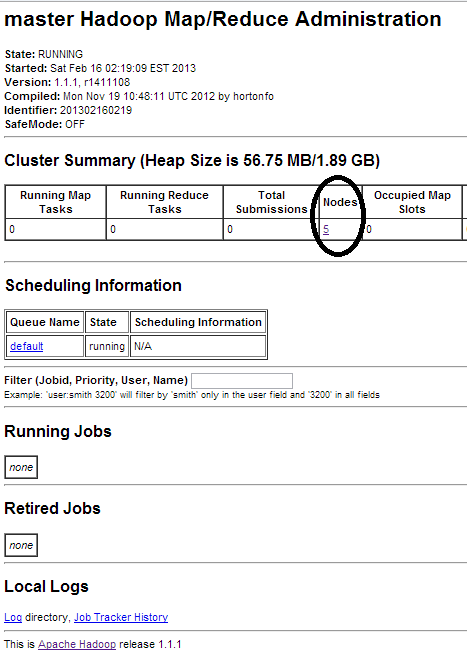
\includegraphics[width=.6\textwidth]{figs/5163os_03_02.png}
  \caption{Hadoop Jobtracker Web UI}\label{fig:jobtracker.webui}
\end{figure} 
The webpage shows that the Hadoop cluster contains 5 active slave nodes.

Check the status each slave node by clicking the link, which lead us to a webpage similar to the following screenshot:
\begin{figure}[ht]
  \centering
  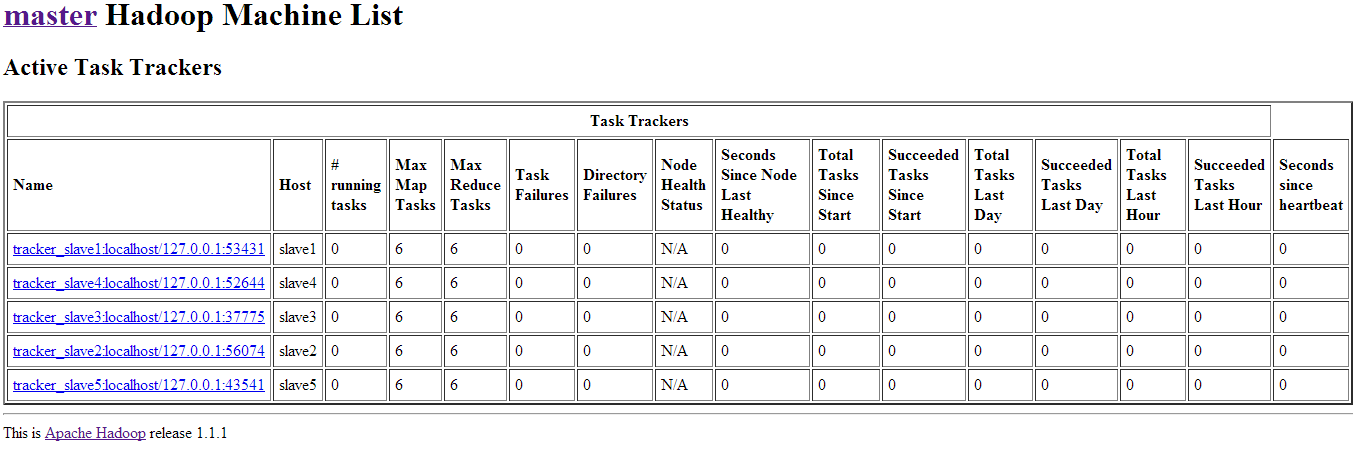
\includegraphics[width=.8\textwidth]{figs/5163os_03_03.png}
  \caption{List of active TaskTrackers}\label{fig:active.trackers}
\end{figure} 
From this screenshot, we can easily check the status of the active TaskTrackers on the slave nodes. For example, we can see the count of failed tasks, the number of MapReduce slots and the heart beat seconds etc.

Check the status of slave DataNodes by opening URL master:50070. The webpage will be similar to the following screenshot: 
\begin{figure}[ht]
  \centering
  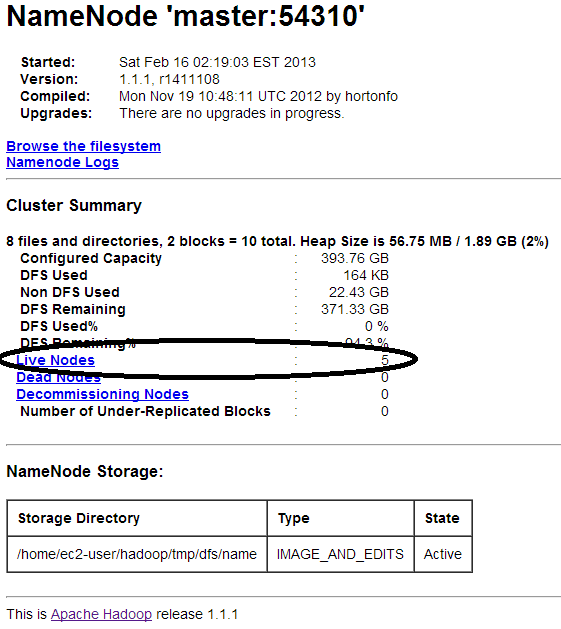
\includegraphics[width=.6\textwidth]{figs/5163os_03_04.png}
  \caption{Hadoop HDFS NameNode Web UI}\label{fig:namenode.webui}
\end{figure} 
The webpage shows that the cluster is configured with 5 active nodes.

By clicking the \verb|``Live Nodes''| link we can see the details of each node as shown in the following screenshot:
\begin{figure}[h]
  \centering
  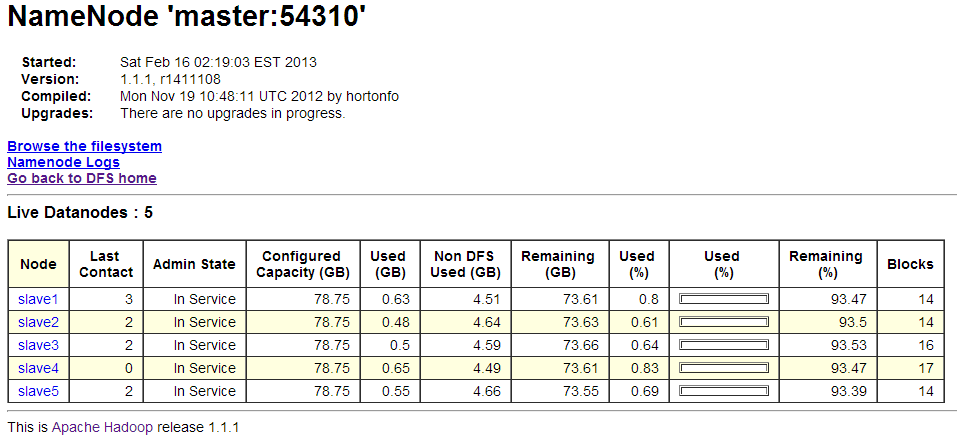
\includegraphics[width=.8\textwidth]{figs/5163os_03_05.png}
  \caption{List of HDFS live DataNodes}\label{fig:hdfs.datanodes}
\end{figure} 
This webpage shows the status of each slave node including node capacity, percentage of usage and how many blocks are hosted in the node etc.

Run an example teragen job to generate 10GB data on the HDFS with command:
\lstset{style=bashstyle}
\begin{lstlisting}
$ hadoop jar $HADOOP_HOME/hadoop-examples-1.1.2.jar teragen $((1024*1024*1024* 10/100)) teraout
\end{lstlisting}

In this command, hadoop-examples-1.1.2.jar is the Java archive file which provides a number of Hadoop examples. The option \verb|$((1024*1024*1024* 10/100))| tells us how many lines of data will be generated with the total data size 10GB.

When the job is running, we can check the status of the job by opening URL \href{http://master:50030/jobdetails.jsp?jobid=job_201302160219_0003&refresh=30}{here}.

In this URL, \verb|job_201302160219_0003| is the job ID and refresh=30 tells how often the webpage should be refreshed.

The job status webpage will be similar to the following screenshot:
\begin{figure}[ht]
  \centering
  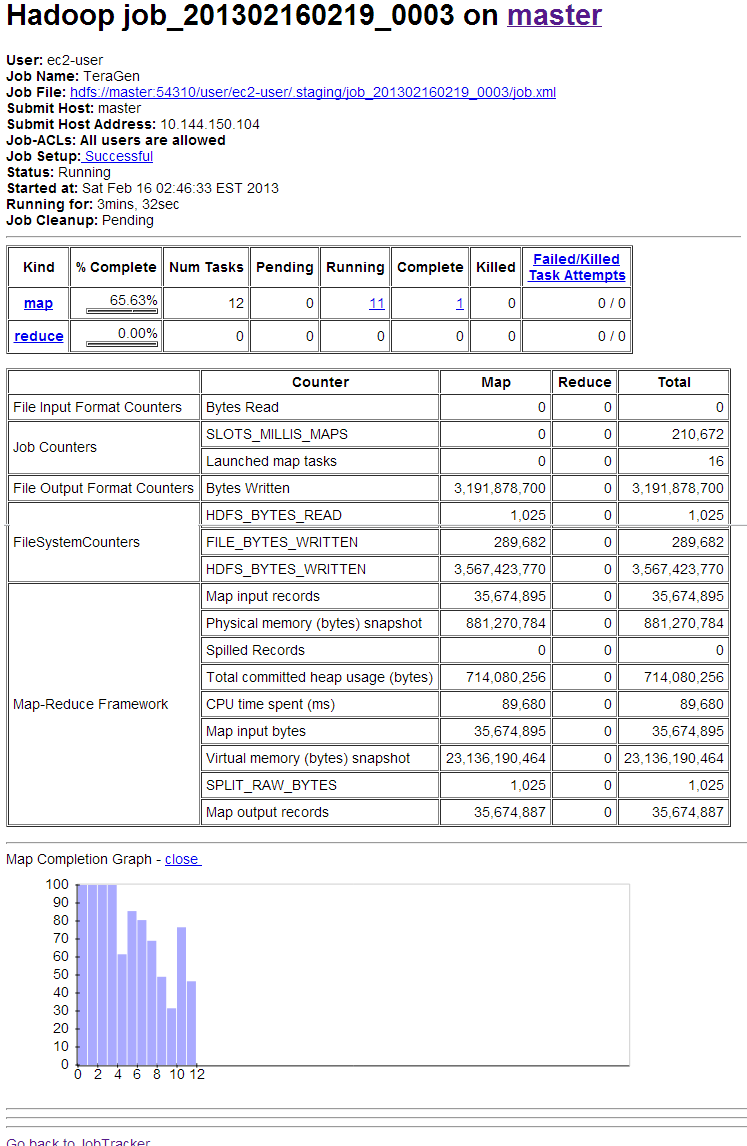
\includegraphics[width=.5\textwidth]{figs/5163os_03_06.png}
  \caption{Information about a MapReduce job from the Web UI}\label{fig:mapreduce.job}
\end{figure} 
This screenshot tells us that the Hadoop cluster has been configured successfully!

After the teragen job finishes, we can check the node storage space usage by opening URL \url{http://master:50070/dfsnodelist.jsp?whatNodes=LIVE}. The webpage will be similar to the following screenshot: \\
\begin{figure}[ht]
  \centering
  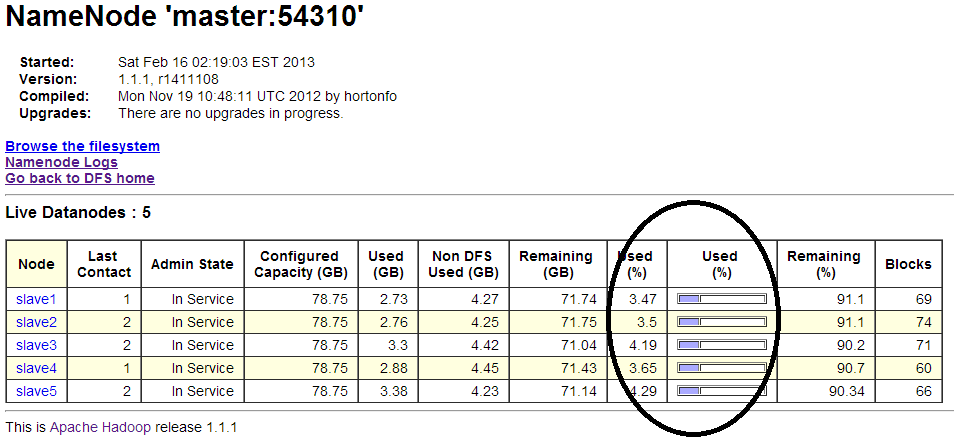
\includegraphics[width=.8\textwidth]{figs/5163os_03_07.png}
  \caption{Storage information of DataNodes from the Web UI}\label{fig:hdfs.storage}
\end{figure} 
The webpage shows that a certain percentage of storage space has been used on each slave node.

Sometimes, a command line based web browser can be more handy than a GUI browser, for example, we can use command \verb|elinks master:50030| to check the status of MapReduce on the master node and use command \verb|elinks master:50070| to check the status and health of HDFS.

Use the following recipe to validate the configuration a Hadoop cluster from command line:

List all available TaskTrackers with command:
\lstset{style=bashstyle}
\begin{lstlisting}[caption=Displaying all active trackers in the MapReduce cluster]
$ hadoop job -list-active-trackers
Example output is similar to the following:
tracker_slave1:localhost/127.0.0.1:53431
tracker_slave4:localhost/127.0.0.1:52644
tracker_slave3:localhost/127.0.0.1:37775
tracker_slave2:localhost/127.0.0.1:56074
tracker_slave5:localhost/127.0.0.1:43541
\end{lstlisting}

The output confirms that all the configured TaskTrackers are active in the Hadoop cluster.

Check the status of HDFS cluster with command:
\lstset{style=bashstyle}
\begin{lstlisting}[caption=Checking the status of the HDFS cluster.]
$ hadoop fsck /
FSCK started by hduser from /10.0.0.1 for path / at Sat Feb 16 03:03:44 EST 2013
...............................Status: HEALTHY
 Total size:    7516316665 B
 Total dirs:    15
 Total files:   31
 Total blocks (validated):      125 (avg. block size 60130533 B)
 Minimally replicated blocks:   125 (100.0 %)
 Over-replicated blocks:        0 (0.0 %)
 Under-replicated blocks:       0 (0.0 %)
 Mis-replicated blocks:         0 (0.0 %)
 Default replication factor:    2
 Average block replication:     2.0
 Corrupt blocks:                0
 Missing replicas:              0 (0.0 %)
 Number of data-nodes:          5
 Number of racks:               1
FSCK ended at Sat Feb 16 03:03:44 EST 2013 in 12 milliseconds


The filesystem under path '/' is HEALTHY
\end{lstlisting}

The output gives us the same information as from the web interface. And the last line tells us that the root filesystem is \emph{HEALTHY}.
\subsection*{How it works}
Hadoop provides commands and web interfaces for system administrators to check the status of the cluster. When we start Hadoop daemons, a build-in web server will be started and a number of pre-written \emph{jsp} script files are used to respond to user's requests from a web browser. The jsp files can be found under the \verb|$HADOOP_HOME/webapps| directory. If you have programming experience, you can take advantage of the jsp files to develop personalized Hadoop cluster management tools.

\subsection*{There's more...}
In this part, we list a few typical Hadoop configuration problems\index{Hadoop configuration problems} and give suggestions on dealing with these problems.

\subsubsection*{Can't start HDFS daemons}
There are many possible reasons that can cause this problem. For example, the NameNode on the master node has not been formatted, in which case, we can format the HDFS before starting the cluster with command: \\
\verb|$ hadoop namenode -format|
\begin{warning}
Warning! \\
Be cautious when formatting the filesystem with this command. It will erase all the data on the file system. Always try other methods before using this one.
\end{warning}

More generically, to troubleshoot this problem, we need to check if HDFS has been properly configured and daemons are running. This can be done with the following command: \\
\verb|$ jps|

If the output of this command \emph{does not} contain the NameNode and SecondaryNameNode daemons, we need to check the configuration of HDFS.

To troubleshoot\index{troubleshoot} the HDFS startup problem, we can open a new terminal and monitor the NameNode log file on the master node with the following command:
\lstset{style=bashstyle}
\begin{lstlisting}
$ tail -f $HADOOP_HOME/logs/hadoop-hduser-namenode-master.log
\end{lstlisting}

This command will show the content of the log file in a dynamic way when new log is appended to the file. If error happens, we can get error messages similar to the following:
\lstset{style=bashstyle}
\begin{lstlisting}[caption=Snippet of the NameNode log on the master node.]
2013-02-16 11:44:29,860 ERROR org.apache.hadoop.hdfs.server.namenode.NameNode: java.net.UnknownHostException: Invalid hostname for server: master1
        at org.apache.hadoop.ipc.Server.bind(Server.java:236)
        at org.apache.hadoop.ipc.Server$Listener.<init>(Server.java:302)
        at org.apache.hadoop.ipc.Server.<init>(Server.java:1488)
        at org.apache.hadoop.ipc.RPC$Server.<init>(RPC.java:560)
        at org.apache.hadoop.ipc.RPC.getServer(RPC.java:521)
        at org.apache.hadoop.hdfs.server.namenode.NameNode.initialize(NameNode.java:295)
        at org.apache.hadoop.hdfs.server.namenode.NameNode.<init>(NameNode.java:529)
        at org.apache.hadoop.hdfs.server.namenode.NameNode.createNameNode(NameNode.java:1403)
        at org.apache.hadoop.hdfs.server.namenode.NameNode.main(NameNode.java:1412)

2013-02-16 11:44:29,865 INFO org.apache.hadoop.hdfs.server.namenode.NameNode: SHUTDOWN_MSG:
/************************************************************
SHUTDOWN_MSG: Shutting down NameNode at master/10.144.150.104
************************************************************/
\end{lstlisting}

Alternatively, the following command will give the same error: \\
\verb|$ hadoop jobtracker|

The message above shows that the hostname of the NameNode is wrong. It should be master instead of master1.

\subsubsection*{Cluster is missing slave nodes}
Most probably, this problem is caused by hostname resolution. To confirm, we can check the content of file \verb|/etc/hosts| with:
\lstset{style=bashstyle}
\begin{lstlisting}
$ cat /etc/hosts
10.0.0.1	master
10.0.0.2	slave1
10.0.0.3	slave2
10.0.0.4	slave3
10.0.0.5	slave4
10.0.0.6	slave5
\end{lstlisting}

If the IP address and hostname mapping does not exist or has been erroneously specified in this file, correcting the error can solve this problem.
\subsubsection*{MapReduce daemons can't be started}
The following two reasons can cause this problem:

The HDFS daemons are not running, which can cause the MapReduce daemons to ping the NameNode daemon at a regular interval, which can be illustrated with the following log output:
\lstset{style=bashstyle}
\begin{lstlisting}
13/02/16 11:32:19 INFO ipc.Client: Retrying connect to server: master/10.0.0.1:54310. Already tried 0           time(s); retry policy is RetryUpToMaximumCountWithFixedSleep(maxRetries=10, sleepTime=1 SECONDS)
13/02/16 11:32:20 INFO ipc.Client: Retrying connect to server: master/10.0.0.1:54310. Already tried 1 time(s); retry policy is RetryUpToMaximumCountWithFixedSleep(maxRetries=10, sleepTime=1 SECONDS)
13/02/16 11:32:21 INFO ipc.Client: Retrying connect to server: master/10.0.0.1:54310. Already tried 2 time(s); retry policy is RetryUpToMaximumCountWithFixedSleep(maxRetries=10, sleepTime=1 SECONDS)
13/02/16 11:32:22 INFO ipc.Client: Retrying connect to server: master/10.0.0.1:54310. Already tried 3 time(s); retry policy is RetryUpToMaximumCountWithFixedSleep(maxRetries=10, sleepTime=1 SECONDS)
13/02/16 11:32:23 INFO ipc.Client: Retrying connect to server: master/10.0.0.1:54310. Already tried 4 time(s); retry policy is RetryUpToMaximumCountWithFixedSleep(maxRetries=10, sleepTime=1 SECONDS).
\end{lstlisting}

To troubleshoot this problem, we can refer to tips for \textbf{can't start HDFS daemons}.

\emph{Configuration problems of MapReduce}. Recall that we have configurations for the number of map slots and reduce slots as well as memory amount in the \verb|$HADOOP_HOME/conf/mapred-site.xml| file. Before starting a cluster, we need to make sure that the total amount of configured memory should be smaller than the total amount of system memory.

For example, suppose a slave host has 4GB of memory, and we have configured 6 map slots and 6 reduce slots with memory 512MB for each slot. So we can compute the total configured task memory with the following formula:  $6 \time 512 + 6 \times 512 = 6GB$.

As 6GB is larger than the system memory 4GB, the system will not start. To clear this problem, we can decrease the number of map slots and reduce slot from 6 to 3. This configuration gives us a total configured memory of 3GB, which is smaller than the system total memory 4GB, thus the MapReduce daemons should be able to start successfully.

\subsection*{See also}
\begin{itemize}
\item Configuring Hadoop in pseudo-distributed mode
\item Configuring Hadoop in fully-distributed mode
\end{itemize}

\section{Configuring ZooKeeper}
ZooKeeper provides highly reliable centralized service for maintaining configuration information, naming and providing distributed synchronization and group services. In this recipe, we will outline steps to install ZooKeeper.

\subsection*{Getting ready}
Make sure Hadoop has been properly configured. Please refer to the previous recipes in this chapter about installation of Hadoop on a cluster.

Login to the master node from the Hadoop administrator machine as hduser with command: \\
\verb|$ ssh hduser@master|

Download ZooKeeper archive file with commands:
\lstset{style=bashstyle}
\begin{lstlisting}
$ wget http://www.gtlib.gatech.edu/pub/apache/zookeeper/stable/zookeeper-3.4.5.tar.gz -P ~/repo
\end{lstlisting}

\subsection*{How to do it...}
Use the following recipe to configure ZooKeeper:

Login to the master node with command: \\
\verb|$ ssh hduser@master|

Copy the downloaded archive to /usr/local with command: 
\lstset{style=bashstyle}
\begin{lstlisting}
$ sudo wget ftp://hadoop.admin/repo/zookeeper-3.4.5.tar.gz -P /usr/local
\end{lstlisting}

De-compress the file with command:
\lstset{style=bashstyle}
\begin{lstlisting}
$ cd /usr/local/
$ sudo tar xvf zookeeper-3.4.5.tar.gz
\end{lstlisting}

Create symbolic link with command:
\lstset{style=bashstyle}
\begin{lstlisting}
$ sudo ln -s /usr/local/zookeeper-3.4.5 /usr/local/zookeeper
\end{lstlisting}

Open file \verb|~/.bashrc| and add the following lines: 
\lstset{style=bashstyle}
\begin{lstlisting}
ZK_HOME=/usr/local/zookeeper
export PATH=$ZK_HOME/bin:$PATH
\end{lstlisting}

Load the configuration file with: \\
\verb|$ . ~/.bashrc|

Create data and log directories for ZooKeeper with command:
\lstset{style=bashstyle}
\begin{lstlisting}
$ sudo mkdir -pv /hadoop/zookeeper/{data,log}
\end{lstlisting}

Create Java configuration file \verb|$ZK_HOME/conf/java.env| with the following content:
\lstset{style=bashstyle}
\begin{lstlisting}
JAVA_HOME=/usr/java/latest
export PATH=$JAVA_HOME/bin:$PATH
\end{lstlisting}

The file name \emph{java.env} is mandatory. It will be loaded by zookeeper.

Create file \verb|$ZK_HOME/conf/zookeeper.cfg| and add the following lines:
\lstset{style=bashstyle}
\begin{lstlisting}
tickTime=2000
clientPort=2181
initLimit=5
syncLimit=2
server.1=master:2888:3888
server.2=slave1:2888:3888
server.3=slave2:2888:3888
server.4=slave3:2888:3888
server.5=slave4:2888:3888
server.6=slave5:2888:3888
dataDir=/hadoop/zookeeper/data
dataLogDir=/hadoop/zookeeper/log
\end{lstlisting}

The highlighted section makes every node know the other nodes in the ZooKeeper ensemble.

Configure ZooKeeper on all slave nodes with command:
\lstset{style=bashstyle}
\begin{lstlisting}
for host in `cat $HADOOP_HOME/conf/slaves`; do
  echo "Configuring ZooKeeper on " $host
  scp ~/.bashrc hduser@$host:~/
  sudo scp -r /usr/local/zookeeper-3.4.5 hduser@$host:/usr/local/
  echo "Making symbolic link for ZooKeeper home directory on " $host
  sudo ssh hduser@$host -C "ln -s /usr/local/zookeeper-3.4.5 /usr/local/zookeeper"
done
\end{lstlisting}

Start ZooKeeper on master node with command: \\
\verb|$ zkServer.sh start|

Verify ZooKeeper configuration with command: \\
\verb|$ zkCli.sh -server master:2181|

Stop ZooKeeper with command: \\
\verb|$ zkServer.sh stop|

\subsection*{See also}
\begin{itemize}
  \item Installing HBase
  \item Get more documentation about ZooKeeper from \href{http://zookeeper.apache.org/doc/r3.4.5/zookeeperAdmin.html}{ZooKeeper Admin Documents}
\end{itemize}

\section{Installing HBase}
HBase is the database based on Hadoop. It is a distributed, scalable Big Data storage system. In this section, we are going to list steps about installing HBase in our Hadoop cluster.

\subsection*{Getting ready}
To install HBase, we assume Hadoop has been configured without any issues.

Download HBase from a mirror site. Similar to downloading Hadoop, HBase is hosted on mirrors all over the world. Visit link \url{http://www.apache.org/dyn/closer.cgi/hbase/} and select the nearest mirror (the suggested mirror on the top is the optimal choice).  After selecting the mirror, follow the link to select the HBase version, we suggest the stable version, for example, follow the link \url{http://mirror.quintex.com/apache/hbase/stable/} and can see the downloadable files as shown in the following screenshot:
\begin{figure}[ht]
  \centering
  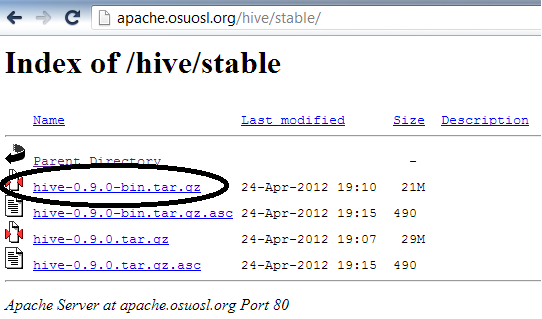
\includegraphics[width=.6\textwidth]{figs/5163os_03_08.png}
  \caption{Download a stable HBase release from a mirror site}\label{fig:hbase.download}
\end{figure} 
Click the file link hbase-0.94.5.tar.gz to download the file to the administrator machine. Then, copy the file to the FTP repository with command: \\
\verb|$ cp hbase-0.94.5.tar.gz ~/repo|

Alternatively, we can download the file with command:
\lstset{style=bashstyle}
\begin{lstlisting}
$ wget http://mirror.quintex.com/apache/hbase/stable/hbase-0.94.5.tar.gz -P ~/repo
\end{lstlisting}

\subsection*{How to do it...}
Use the following recipe to install HBase: \\
Login to the master node from administrator machine with command: \\
\verb|$ ssh hduser@master|

De-compress the HBase archive with commands:
\lstset{style=bashstyle}
\begin{lstlisting}
$ cd /usr/local
$ sudo wget ftp://hadoop.admin/repo/hbase-0.94.5.tar.gz -P /usr/local
$ sudo tar xvf hbase-0.94.5.tar.gz
\end{lstlisting}

Create symbolic link with command: \\
\verb|$ ln -s hbase-0.94.5 hbase|

Use your favorite text editor to open file ~/.bashrc and append the following lines into the file:
\begin{verbatim}
export HBASE_HOME=/usr/local/hbase
export PATH=$HBASE_HOME/bin:$PATH
\end{verbatim}

Open file \verb|$HBASE_HOME/conf/hbase-env.sh| and set \verb|JAVA_HOME| as: \\
\verb|$ export JAVA_HOME=/usr/java/latest|

Open file \verb|$HBASE_HOME/conf/hbase-site.xml| with your favorite text editor and add the following contents to the file:
\lstset{style=bashstyle}
\begin{lstlisting}
<?xml version="1.0"?>
<?xml-stylesheet type="text/xsl" href="configuration.xsl"?>
<configuration>
  <property>
    <name>hbase.rootdir</name>
    <value>hdfs://master:54310/hbase</value>
  </property>

  <property>
    <name>hbase.cluster.distributed</name>
    <value>true</value>
  </property>

  <property>
    <name>hbase.tmp.dir</name>
    <value>/hadoop/hbase</value>
  </property>

  <property>
    <name>hbase.ZooKeeper.quorum</name>
    <value>master</value>
  </property>

  <property>
    <name>hbase.zookeeper.property.dataDir</name>
    <value>/hadoop/zookeeper</value>
  </property>
</configuration>
\end{lstlisting}

Open file \verb|$HBASE_HOME/conf/regionservers| and add the following lines:
\begin{verbatim}
slave1
slave2
slave3
slave4
slave5
\end{verbatim}

Link the HDFS configure file to HBase configuration directory with command:
\lstset{style=bashstyle}
\begin{lstlisting}
$ sudo ln -s $HADOOP_HOME/conf/hdfs-site.xml $HBASE_HOME/conf/hdfs-site.xml
\end{lstlisting}

Replace the dependent jar files for HBase with command:
\lstset{style=bashstyle}
\begin{lstlisting}
$ rm -i $HBASE_HOME/lib/hadoop-core*.jar $HBASE_HOME/lib/zookeeper-*.jar
$ cp -i $HADOOP_HOME/hadoop-core*.jar $HADOOP_HOME/lib/commons-*.jar $ZK_HOME/zookeeper-*.jar $HBASE_HOME/lib/
\end{lstlisting}

Configure all the slave nodes with command:
\lstset{style=bashstyle}
\begin{lstlisting}
for host in `cat $HBASE_HOME/conf/regionservers`; do
  echo "Configuring HBase on " $host
  scp ~/.bashrc hduser@$host:~/
  sudo scp -r /usr/local/hbase-0.94.5 hduser@$host:/usr/local/
  echo "Making symbolic link for HBase home directory on " $host
  sudo ssh hduser@$host -C "ln -s /usr/local/hbase-0.94.5 /usr/local/hbase"
  echo "Making symbolic link for hdfs-site.xml to the HBase configuration directory on " $host
  sudo ssh hduser@$host -C "ln -s /usr/local/hadoop-1.1.2/conf/hdfs-site.xml /usr/local/hbase-0.94.5/conf/hdfs-site.xml"
done
\end{lstlisting}

Start HBase daemons with command: \\
\verb|$ start-hbase.sh|

Connect to the running HBase with command: \\
\verb|$ hbase shell|

Verify the HBase installation with the following HBase shell commands: 
\lstset{style=bashstyle}
\begin{lstlisting}
hbase(main):001:0> create 'test', 'c'
0 row(s) in 0.2410 seconds

hbase(main):001:0> put 'test', 'r1', 'c:a', 'v1'
0 row(s) in 0.0320 seconds

hbase(main):003:0> scan 'test'
ROW COLUMN+CELL row1 column=c:a, timestamp=124455459102, value=v1 r1
1 row(s) in 0.2130 seconds

hbase(main):006:0> disable 'test'
0 row(s) in 9.4210 seconds

hbase(main):007:0> drop 'test'
0 row(s) in 8.3412 seconds

hbase(main):010:0> exit
\end{lstlisting}

To stop HBase, use command:
\begin{verbatim}
$ stop-hbase.sh
stopping hbase...............
\end{verbatim}

\subsection*{How it works}
In the configuration, property hbase.rootdir specifies the root directory of the HBase data storage. And property \emph{hbase.zookeeper.property.dataDir} specifies the root directory of the ZooKeeper data storage.

\subsection*{There's more...}
\begin{itemize}
  \item Installing ZooKeeper in Chapter 3, Configuring a Hadoop cluster
  \item More documentation about HBase can be found \href{http://wiki.apache.org/hadoop/Hbase}{here}
\end{itemize}

\section{Installing Hive}
As a top level abstraction language, Hive provides a handy tool for manipulating data storage on HDFS with SQL like language. In this section, we will talk about installing Hive on our Hadoop cluster.

\subsection*{Getting ready}
Before we install Hive, we need to make sure Hadoop has been properly installed. Please refer to the previous sections about the configuration of a Hadoop cluster. \\
Download Hive from a mirror site with command similar to the following on the administrator machine:
\lstset{style=bashstyle}
\begin{lstlisting}
$ wget http://apache.osuosl.org/hive/stable/hive-0.9.0.tar.gz -P ~/repo
\end{lstlisting}

\subsection*{How to do it...}
Use the following steps to install Hive:

Login to the master node from the Hadoop administrator machine as hduser with command: \\
\verb|$ ssh hduser@master|

Copy the archive to /usr/local with command:
\lstset{style=bashstyle}
\begin{lstlisting}
$ sudo wget ftp://hadoop.admin/repo/hive-0.9.0.tar.gz /usr/local
\end{lstlisting}

De-compress the Hive archive with command:
\lstset{style=bashstyle}
\begin{lstlisting}
$ cd /usr/local
$ tar xvf hive-0.9.0.tar.gz
\end{lstlisting}

Create symbolic link with command:
\lstset{style=bashstyle}
\begin{lstlisting}
$ ln -s /usr/local/hive-0.9.0 /usr/local/hive
\end{lstlisting}

Use your favorite text editor to open file \verb|~/.bashrc| and add the following lines to this file:
\lstset{style=bashstyle}
\begin{lstlisting}
export HIVE_HOME=/usr/local/hive
export PATH=$HIVE_HOME/bin:$PATH
\end{lstlisting}

Start Hive with command: \\
\verb|$ hive|
\subsection*{There's more...}
\begin{itemize}
  \item Installing Pig in Chapter 3, Configuring a Hadoop cluster
  \item Get more documentation about Hive from \href{https://cwiki.apache.org/confluence/display/Hive/Home}{Hive Home}
\end{itemize}

\section{Installing Pig}
Similar to Hive, Pig provides a handy tool for manipulating Hadoop data. In this recipe, we are going to discuss the installation of Apache Pig.
\subsection*{Getting ready}
Before we install Pig, we need to make sure Hadoop has been properly installed. Please refer to the previous sections about the configuration of a Hadoop cluster.

Download Pig the archive file from a mirror site with command on the administrator machine:
\lstset{style=bashstyle}
\begin{lstlisting}
$ wget http://www.motorlogy.com/apache/pig/stable/pig-0.10.1.tar.gz ~/repo
\end{lstlisting}

\subsection*{How to do it...}
Use the following steps to configure Pig:

Login to the master node from the Hadoop administrator machine as hduser with command: \\
\verb|$ ssh hduser@master|

Copy the archive to \verb|/usr/local| with the following command: 
\lstset{style=bashstyle}
\begin{lstlisting}
$ sudo wget ftp://hadoop.admin/repo/pig-0.10.1.tar.gz /usr/local
\end{lstlisting}

De-compress the Pig archive file with command:
\lstset{style=bashstyle}
\begin{lstlisting}
$ cd /usr/local
$ sudo tar xvf pig-0.10.1.tar.gz
\end{lstlisting}

Create symbolic link to the Pig directory:
\lstset{style=bashstyle}
\begin{lstlisting}
$ sudo ln -s /usr/local/pig-0.10.1 /usr/local/pig
\end{lstlisting}

Open file ~/.bashrc with your favorite text editor and add the following lines into the file:
\lstset{style=bashstyle}
\begin{lstlisting}
export PIG_HOME=/usr/local/pig
export PATH=$PIG_HOME/bin:$PATH
\end{lstlisting}

Run Pig in local mode with command: \\
\verb|$ pig -x local|

Run Pig in MapReduce mode with command: \\
\verb|$ pig|

Alternatively, we can use the following command: \\
\verb|$ pig -x mapreduce| \\
Pig that runs in MapReduce mode will utilizes the power of distributed computing provided by Hadoop.

\subsection*{There's more...}
\begin{itemize}
  \item Installing Hive in Chapter 3, Configuring a Hadoop cluster
  \item More documentation about Pig can be obtained from \href{http://pig.apache.org/docs/r0.10.0/}{Pig @ Apache}
\end{itemize}

\section{Installing Mahout}
Apache Mahout is a machine learning library that scales machine learning algorithms on Big Data. It is implemented on top of the Hadoop Big Data stack. It already has implementation of a wide range of machine learning algorithms. In this recipe, we will outline steps to configure Apache Mahout.
\subsection*{Getting ready}
Before we install Mahout, we need to make sure Hadoop has been properly installed.

Download Mahout from the mirror site with the following command on the master node:
\lstset{style=bashstyle}
\begin{lstlisting}
$ wget http://www.eng.lsu.edu/mirrors/apache/mahout/0.7/mahout-distribution-0.7.tar.gz -P ~/repo
\end{lstlisting}

\subsection*{How to do it...}
Use the following the recipe to install Mahout:
Login to the master node from the Hadoop administrator machine as hduser with command: \\
\verb|$ ssh hduser@master|

Copy the archive to /usr/local with command:
\lstset{style=bashstyle}
\begin{lstlisting}
$ sudo wget ftp://hadoop.admin/repo/mahout-distribution-0.7.tar.gz /usr/local
\end{lstlisting}

De-compress the Mahout archive with command: 
\lstset{style=bashstyle}
\begin{lstlisting}
$ cd /usr/local
$ sudo tar xvf mahout-distribution-0.7.tar.gz
\end{lstlisting}

Create symbolic link to the Mahout directory with command: 
\lstset{style=bashstyle}
\begin{lstlisting}
$ sudo ln -s /usr/local/mahout-distribution-0.7 /usr/local/mahout 
\end{lstlisting}

Open file ~/.bashrc with your favorite text editor and add the following lines to the file: \\
\verb|export MAHOUT_HOME=/usr/local/pig| \\
\verb|export PATH=$MAHOUT_HOME/bin:$PATH|

Load the configuration with command: \\
\verb|$ . ~/.bashrc| \\

Install Maven with command: \\
\verb|$ sudo yum install maven|

Compile and install Mahout core with the following commands:
\lstset{style=bashstyle}
\begin{lstlisting}
$ cd $MAHOUT_HOME
$ sudo mvn compile
$ sudo mvn install
\end{lstlisting}

The install command will run all the tests by default, we can ignore the tests to speed up the installation process with command sudo mvn -DskipTests install.

Compile the Mahout examples with commands:
\lstset{style=bashstyle}
\begin{lstlisting}
$ cd examples
$ sudo mvn compile
\end{lstlisting}

Use the following steps to verify Mahout configuration:

Download sample data with command:
\lstset{style=bashstyle}
\begin{lstlisting}
$ wget http://archive.ics.uci.edu/ml/databases/synthetic_control/synthetic_control.data -P ~/
\end{lstlisting}

Start the Hadoop cluster with commands:
\lstset{style=bashstyle}
\begin{lstlisting}
$ start-dfs.sh
$ start-mapred.sh
\end{lstlisting}

Put the downloaded data into HDFS with commands:
\lstset{style=bashstyle}
\begin{lstlisting}
$ hadoop fs -mkdir testdata
$ hadoop fs -put ~/synthetic_control.data testdata
\end{lstlisting}

Run kmeans clustering with command:
\lstset{style=bashstyle}
\begin{lstlisting}$ mahout org.apache.mahout.clustering.syntheticcontrol.kmeans.Job
\end{lstlisting}

\subsection*{There's more...}
\begin{itemize}
  \item More documentation about Mahout can be obtained from the \href{https://cwiki.apache.org/confluence/display/MAHOUT/Mahout+Wiki}{Mahout Wiki}
\end{itemize}
